%% Online Resource 1 (electronic supplementary material) for the Research in Engineering Design manuscript.
\documentclass[pdflatex,sn-chicago]{sn-jnl}

\usepackage{graphicx}
\usepackage{multirow}
\usepackage{amsmath,amssymb,amsfonts}
\usepackage{booktabs}
\usepackage{siunitx}
\usepackage{manyfoot}
\graphicspath{{figures/}}
\raggedbottom
\renewcommand{\thetable}{S\arabic{table}}
\renewcommand{\thefigure}{S\arabic{figure}}
\renewcommand{\thesection}{S\arabic{section}}
\renewcommand{\topfraction}{0.9}
\renewcommand{\textfraction}{0.07}
\renewcommand{\floatpagefraction}{0.8}
\setcounter{totalnumber}{4}

\begin{document}

\title[Online Resource 1]{Online Resource 1: supplementary material for ``Alternative-dependent diagnosability: co-selecting system architecture and monitoring suite under a detectability requirement, demonstrated on three wind-turbine generator topologies''}

\author*[1]{\fnm{H\"useyin Tayyer} \sur{Canseven}}\email{huseyin.canseven@lut.fi}
\affil*[1]{\orgdiv{Department of Electrical Engineering, LUT School of Energy Systems}, \orgname{LUT University}, \orgaddress{\street{Yliopistonkatu 34}, \city{Lappeenranta}, \postcode{53850}, \country{Finland}}}

\abstract{This supplement contains the feature definitions (Section~S1), the computation details of the demonstration (Section~S2), the supplementary tables S1--S12 and the supplementary figures S1--S2 referred to in the main text. Every table and figure is produced by the released code from the public datasets.}

\keywords{supplementary material}

\maketitle

\section{Feature definitions}\label{s:features}

Let $x_a, x_b, x_c$ be the sampled phase quantities of a window of $N$ samples at sampling frequency $f_s$, $w$ the Hann window and $f_e$ the electrical frequency of the window. The complex fundamental amplitude of a signal $x$ at frequency $f$ is
\begin{equation}
  X(f) = \frac{2}{\sum_n w_n}\sum_{n=0}^{N-1} x_n\, w_n\, e^{-j2\pi f n/f_s}.
\end{equation}
The electrical frequency is estimated from the slope of the unwrapped phase of the current space vector $\tfrac{2}{3}(i_a + \mathbf{a}\, i_b + \mathbf{a}^2 i_c)$, $\mathbf{a}=e^{j2\pi/3}$, whose sign gives the phase rotation; outside 0.5--1.5 times the nominal value the nominal value is used. Sequence magnitudes are $|X_+| = |X_a + \mathbf{a}X_b + \mathbf{a}^2X_c|/3$ and $|X_-| = |X_a + \mathbf{a}^2X_b + \mathbf{a}X_c|/3$ for an $abc$ rotation (interchanged for $acb$), evaluated at $f=f_e$ for currents ($I_1, I_2$), terminal voltages ($V_1, V_2$) and mean-removed duty cycles ($D_1, D_2$); $|X(f)|$ is a fundamental amplitude (peak) and is divided by $\sqrt2$ wherever it is compared with an RMS value. The RMS unbalance is $\max_k |I_{\mathrm{rms},k} - \bar I_{\mathrm{rms}}| / \bar I_{\mathrm{rms}}$ over the three phases. Harmonic ratios are $|I_a(kf_e)|/|I_a(f_e)|$ for $k=3,5,7$, and the THD is $\sqrt{\sum_{k=2}^{20}|I_a(kf_e)|^2}/|I_a(f_e)|$. For the synchronous-frame currents $i_d, i_q$ and the torques the features are the standard deviation of the mean-removed signal and its amplitudes $|Y(f_e)|$ and $|Y(2f_e)|$; for the PI outputs the standard deviation and $|Y(2f_e)|$; for the measured and commanded synchronous-frame voltages $|Y(2f_e)|$ only; for the field current the standard deviation and $|Y(2f_e)|$. Speed and DC-link features are standard deviations. Windows are $n_c$ electrical cycles long with a hop of one cycle; a feature is undefined for a trial whose faulted interval holds no complete window. On the WFSG bench the measured converter-side phase voltages serve as terminal voltages, the synchronous-frame voltages are obtained from them with the encoder angle, the commanded voltages are the controller's, and the electrical torque is computed from power and speed.

\section{Computation details}\label{s:computation}

\paragraph{Intervals.} PMSG and SCIG: reference interval 0.30--0.98\,s after the start of each record, split at 0.62\,s into $R_1$ (0.32\,s) and $R_2$ (0.36\,s); contactor commanded at 1.000\,s; faulted interval from 30\,ms after the command to 10\,ms before its release; the relay picks up 85--90\,ms after the command, so the faulted interval contains about 55\,ms of healthy time (at most 15\,\% of its length); recovery windows start 0.30\,s after the release. WFSG: fault interval located from the measured fault current as the first contiguous interval in which its 10\,ms RMS exceeds $\max(0.3\,\mathrm{A}, 6\sigma)$, $\sigma$ being the standard deviation of that RMS over 0.05--0.40\,s, ending at the first fall below the threshold after 50\,ms; reference interval from 0.05\,s after the start of the record to 10\,ms before the onset, split at 0.30\,s ($R_1$ 0.25\,s, $R_2$ about 0.24\,s); recovery windows start 0.15\,s after the end of the fault interval. At 23.9--63.7\,Hz a WFSG faulted interval holds between zero and eleven three-cycle windows; four trials hold none and are dropped; 81 of 438 hold fewer than three (all 50 trials at 1671\,rpm, 26 of 206 at 1800\,rpm, 4 at 716 and 1 at 955\,rpm).

\paragraph{Null and screen.} The null is pooled over all 225 records of each of the PMSG and SCIG and over the 438 inter-turn and inter-winding records of the WFSG. The reliability screen flags a feature when its count of false alarms on the nine healthy trials is incompatible with the nominal rate $1-\alpha$ at the 5\,\% level (one-sided binomial test: three or more at $\alpha=0.95$, two or more at $\alpha=0.99$, four or more at $\alpha=0.90$), and excludes features whose null quantile exceeds one.

\paragraph{Bootstrap.} 2000 resamples, seed 1. Median SDR and detectable share of a class: cluster bootstrap over the twelve tap pairs, the same resampled pairs for both machines; Wilson 95\,\% intervals for shares. Minimum detectable extent: operating-point trials resampled within each extent level; the limit-of-detection rule applied to each resample. The null quantile is held at its full-sample value. Decision table: 1000 resamples per suite, alternative, class and $\alpha$ (seed 7); a suite \emph{meets} $e_{\mathrm{req}}$ when the resample probability of $\mathrm{MDE}\le e_{\mathrm{req}}$ is at least 0.95 and \emph{fails} when it is at most 0.05.

\paragraph{Transfer.} Windows: reference, faulted and recovery windows of all trials; positives: faulted windows of fault trials. Models: scikit-learn histogram gradient boosting (max depth 3, 200 iterations, learning rate 0.08, random state 0) and logistic regression with standardisation ($C=1$, 3000 iterations). Cross-validation: five-fold GroupKFold with one group per tap pair and machine, healthy trials grouped by speed. Referencing rules: physical units; $z$-score on the target machine's healthy trials; absolute $z$-score against the mean and standard deviation of the first half of the trial's own reference interval (windows starting before 0.62\,s for the PMSG/SCIG, before 0.30\,s for the WFSG). Metrics: AUC and true-positive rate at 1\,\% false-positive rate on all windows and on the windows outside the normalising set; the false-alarm rate of the all-negatives 1\,\% threshold on the fault-time windows of the healthy trials.

\section{Supplementary tables}

\begin{table}[t]
\scriptsize
\caption{Observation suites for the three alternatives, three-cycle windows, common feature set. MDE (\%) at the fault impedance matching the PMSG/SCIG protocol; $^{\dagger}$the smallest inter-turn extent tested on the WFSG at that impedance is 11.6\,\%, so the value is an upper bound. DS: detectable share (\%) of the fixed feature; oracle: per-trial best feature.}\label{tab:suites3}
\begin{tabular}{@{}llllcc@{}}
\toprule
Suite & Machine & Feature & MDE & DS & Oracle DS \\
\midrule
\multicolumn{6}{@{}l}{\emph{Inter-turn faults}} \\
drive-internal & PMSG & $D_2/D_1$ & 7.4 & 65 & 81 \\
drive-internal & SCIG & $V_d^{\mathrm{cmd}}$\,2$f_e$ & 7.4 & 73 & 87 \\
drive-internal & WFSG & $I_q$\,2$f_e$ & 11.6$^{\dagger}$ & 81 & 97 \\
3 CT & PMSG & $I_2/I_1$ & 7.4 & 57 & 79 \\
3 CT & SCIG & $I_2/I_1$ & 7.4 & 70 & 81 \\
3 CT & WFSG & RMS unbal. & 11.6$^{\dagger}$ & 78 & 94 \\
3 CT + 3 VT & PMSG & $I_2/I_1$ & 7.4 & 57 & 79 \\
3 CT + 3 VT & SCIG & $I_2/I_1$ & 7.4 & 70 & 81 \\
3 CT + 3 VT & WFSG & $V_2/V_1$ & 11.6$^{\dagger}$ & 78 & 95 \\
3 CT + 3 VT + drive & PMSG & $D_2/D_1$ & 7.4 & 65 & 92 \\
3 CT + 3 VT + drive & SCIG & $V_d^{\mathrm{cmd}}$\,2$f_e$ & 7.4 & 73 & 94 \\
3 CT + 3 VT + drive & WFSG & $V_2/V_1$ & 11.6$^{\dagger}$ & 78 & 98 \\
excitation (field current) & WFSG & $I_f$\,2$f_e$ & 11.6$^{\dagger}$ & 70 & 76 \\
\multicolumn{6}{@{}l}{\emph{Inter-winding faults}} \\
drive-internal & PMSG & $D_2/D_1$ & 2.3 & 91 & 98 \\
drive-internal & SCIG & $V_d^{\mathrm{cmd}}$\,2$f_e$ & 2.3 & 100 & 100 \\
drive-internal & WFSG & $I_q$\,2$f_e$ & 2.3 & 100 & 100 \\
3 CT & PMSG & $I_2/I_1$ & 9.7 & 83 & 99 \\
3 CT & SCIG & $I_2/I_1$ & 2.3 & 98 & 98 \\
3 CT & WFSG & $I_a$\,h3 & 2.3 & 100 & 100 \\
3 CT + 3 VT & PMSG & $I_2/I_1$ & 9.7 & 83 & 99 \\
3 CT + 3 VT & SCIG & $I_2/I_1$ & 2.3 & 98 & 98 \\
3 CT + 3 VT & WFSG & $I_a$\,h3 & 2.3 & 100 & 100 \\
3 CT + 3 VT + drive & PMSG & $D_2/D_1$ & 2.3 & 91 & 100 \\
3 CT + 3 VT + drive & SCIG & $V_d^{\mathrm{cmd}}$\,2$f_e$ & 2.3 & 100 & 100 \\
3 CT + 3 VT + drive & WFSG & $I_q$\,2$f_e$ & 2.3 & 100 & 100 \\
excitation (field current) & WFSG & $I_f$\,2$f_e$ & 2.3 & 100 & 100 \\
\botrule
\end{tabular}
\end{table}

\begin{table}[t]
\scriptsize
\caption{Five features with the highest median SDR per alternative and fault class (three-cycle windows, all WFSG impedances); detectable share in parentheses (\%).}\label{tab:topfeat}
\begin{tabular}{@{}llp{7.6cm}@{}}
\toprule
Machine & Class & Features: median SDR (DS) \\
\midrule
PMSG & inter-turn & $V_2/V_1$ 2.5 (73); $D_2/D_1$ 2.4 (65); $I_2/I_1$ 1.4 (57); $V_q$\,2$f_e$ 1.2 (55); $V_q^{\mathrm{cmd}}$\,2$f_e$ 1.1 (55) \\
PMSG & inter-winding & $V_2/V_1$ 51.5 (92); $D_2/D_1$ 28.7 (91); $V_q$\,2$f_e$ 19.8 (89); $I_2/I_1$ 11.5 (83); $V_d$\,2$f_e$ 5.6 (71) \\
SCIG & inter-turn & $I_d$\,2$f_e$ 6.5 (78); $V_d^{\mathrm{cmd}}$\,2$f_e$ 5.5 (73); $D_2/D_1$ 5.5 (78); $I_2/I_1$ 4.0 (70); $V_q^{\mathrm{cmd}}$\,2$f_e$ 3.6 (66) \\
SCIG & inter-winding & $I_d$\,2$f_e$ 73.0 (100); $V_d^{\mathrm{cmd}}$\,2$f_e$ 57.3 (100); $D_2/D_1$ 50.7 (100); $I_2/I_1$ 49.5 (98); $V_2/V_1$ 40.7 (100) \\
WFSG & inter-turn & $V_2/V_1$ 9.4 (80); $I_q$\,2$f_e$ 7.3 (82); $V_q^{\mathrm{cmd}}$\,2$f_e$ 7.1 (82); RMS unbal. 5.6 (80); $V_q$\,2$f_e$ 4.9 (81) \\
WFSG & inter-winding & $I_q$\,2$f_e$ 33.0 (100); $V_q^{\mathrm{cmd}}$\,2$f_e$ 31.9 (100); $D_2/D_1$ 26.9 (100); $I_q$\,std 24.3 (95); $I_a$\,h3 21.8 (100) \\
\botrule
\end{tabular}
\end{table}

\begin{table}[t]
\footnotesize
\caption{Operating-point dependence: median SDR of the best of $V_2/V_1$, $V_q$\,2$f_e$, $I_2/I_1$, PI$_d$\,2$f_e$ and detectable share (\%) per cell of the speed--torque grid, 24 fault trials per cell.}\label{tab:opgrid}
\begin{tabular}{@{}llccc@{}}
\toprule
Machine & Speed (rpm) & 5.2\,N\,m & 6.4\,N\,m & 8.0\,N\,m \\
\midrule
PMSG & 1200 & 7.9 / 83 & 9.0 / 83 & 5.3 / 79 \\
PMSG & 1500 & 12.8 / 96 & 11.3 / 96 & 9.6 / 92 \\
PMSG & 1800 & 20.5 / 92 & 18.2 / 96 & 15.5 / 92 \\
SCIG & 1200 & 18.1 / 92 & 16.6 / 92 & 16.1 / 96 \\
SCIG & 1500 & 26.4 / 92 & 23.5 / 92 & 23.8 / 92 \\
SCIG & 1800 & 51.0 / 100 & 47.2 / 100 & 44.0 / 96 \\
\botrule
\end{tabular}
\end{table}

\begin{table}[t]
\scriptsize
\setlength{\tabcolsep}{3pt}
\caption{Sensitivity of MDE (\%)/DS (\%) to the window length (3, 5, 8 cycles at $\alpha=0.95$) and to the null quantile ($\alpha=0.90$ and $0.99$ at five cycles). IT: inter-turn; IW: inter-winding.}\label{tab:sens}
\begin{tabular}{@{}lllccccc@{}}
\toprule
Class & Feature & Machine & 3\,c & 5\,c & 8\,c & $\alpha$\,0.90 & $\alpha$\,0.99 \\
\midrule
IT & $V_2/V_1$ & PMSG & 2.8/73 & 2.8/76 & 2.8/73 & 2.8/80 & 3.8/69 \\
IT & $V_2/V_1$ & SCIG & 7.4/69 & 2.7/73 & 2.7/75 & 2.7/76 & 7.4/65 \\
IT & $I_2/I_1$ & PMSG & 7.4/57 & 7.4/56 & 7.4/58 & 2.8/65 & 7.4/52 \\
IT & $I_2/I_1$ & SCIG & 7.4/70 & 2.8/75 & 2.8/75 & 2.8/79 & 7.4/68 \\
IT & $I_d$\,2$f_e$ & PMSG & 11.6/29 & 11.6/30 & 11.6/28 & 11.6/33 & 11.6/24 \\
IT & $I_d$\,2$f_e$ & SCIG & 2.8/78 & 2.7/79 & 2.7/83 & 2.7/84 & 7.4/72 \\
IT & PI$_d$\,2$f_e$ & PMSG & 11.6/30 & 11.6/31 & 11.6/28 & 11.6/33 & 11.6/24 \\
IT & PI$_d$\,2$f_e$ & SCIG & 2.8/78 & 2.7/78 & 2.7/83 & 2.7/84 & 7.4/72 \\
IT & $V_q$\,2$f_e$ & PMSG & 7.4/55 & 7.4/57 & 7.4/60 & 7.4/65 & 7.4/50 \\
IT & $V_q$\,2$f_e$ & SCIG & 7.4/61 & 7.4/60 & 7.4/62 & 7.4/64 & 7.4/59 \\
IW & $V_2/V_1$ & PMSG & 2.3/92 & 2.3/94 & 2.3/94 & 2.3/94 & 2.3/91 \\
IW & $V_2/V_1$ & SCIG & 2.3/100 & 2.3/100 & 2.3/100 & 2.3/100 & 2.3/100 \\
IW & $I_2/I_1$ & PMSG & 9.7/83 & 9.7/81 & 9.7/82 & 3.2/87 & 9.7/79 \\
IW & $I_2/I_1$ & SCIG & 2.3/98 & 2.3/100 & 2.3/100 & 2.3/100 & 2.3/97 \\
IW & $I_d$\,2$f_e$ & PMSG & 10.6/71 & 10.6/72 & 10.6/69 & 10.6/74 & 14.3/69 \\
IW & $I_d$\,2$f_e$ & SCIG & 2.3/100 & 2.3/100 & 2.3/100 & 2.3/100 & 2.3/100 \\
IW & PI$_d$\,2$f_e$ & PMSG & 10.6/71 & 10.6/72 & 10.6/70 & 10.6/74 & 14.3/69 \\
IW & PI$_d$\,2$f_e$ & SCIG & 2.3/100 & 2.3/100 & 2.3/100 & 2.3/100 & 2.3/100 \\
IW & $V_q$\,2$f_e$ & PMSG & 2.3/89 & 2.3/90 & 2.3/91 & 2.3/91 & 9.7/86 \\
IW & $V_q$\,2$f_e$ & SCIG & 9.7/88 & 2.3/92 & 9.7/88 & 2.3/95 & 9.7/84 \\
\botrule
\end{tabular}
\end{table}

\begin{table}[t]
\scriptsize
\caption{Bootstrap over trials (2000 resamples, 95\,\% percentile intervals): median SDR per machine and ratio of medians SCIG/PMSG. Five-cycle windows, $\alpha=0.95$. Intervals of the detectable shares are in Fig.~\ref{fig:boot}.}\label{tab:boot}
\begin{tabular}{@{}llccc@{}}
\toprule
Class & Feature & PMSG median SDR & SCIG median SDR & SCIG/PMSG \\
\midrule
inter-turn & $V_2/V_1$ & 2.99 [1.62, 5.14] & 4.17 [1.98, 6.61] & 1.32 [0.52, 2.87] \\
inter-turn & $I_2/I_1$ & 1.47 [0.92, 1.78] & 4.52 [2.24, 6.01] & 3.10 [1.60, 5.59] \\
inter-turn & $I_d$\,2$f_e$ & 0.52 [0.42, 0.65] & 6.68 [2.62, 10.20] & 12.61 [5.00, 20.64] \\
inter-turn & PI$_d$\,2$f_e$ & 0.52 [0.42, 0.67] & 6.69 [2.85, 10.27] & 12.49 [5.24, 20.83] \\
inter-turn & $V_q$\,2$f_e$ & 1.35 [0.97, 2.44] & 2.58 [1.54, 3.48] & 2.01 [0.91, 3.18] \\
inter-winding & $V_2/V_1$ & 61.90 [35.54, 91.27] & 48.19 [29.43, 89.07] & 0.83 [0.43, 1.96] \\
inter-winding & $I_2/I_1$ & 11.32 [3.95, 22.16] & 55.61 [36.17, 93.45] & 5.38 [2.41, 16.59] \\
inter-winding & $I_d$\,2$f_e$ & 4.14 [2.49, 6.92] & 73.97 [45.53, 127.88] & 18.00 [9.66, 36.97] \\
inter-winding & PI$_d$\,2$f_e$ & 4.21 [2.51, 7.01] & 74.01 [45.55, 127.95] & 17.78 [9.41, 36.22] \\
inter-winding & $V_q$\,2$f_e$ & 22.40 [10.67, 35.86] & 24.80 [13.75, 36.40] & 1.07 [0.51, 2.44] \\
\botrule
\end{tabular}
\end{table}

\begin{table}[t]
\scriptsize
\setlength{\tabcolsep}{3pt}
\caption{Transfer of a GBDT detector restricted to each suite's features (AUC), PMSG and SCIG, five-cycle windows: features $z$-scored on the target's healthy trials (left block) and $|z|$ against each trial's own reference (right block). P: PMSG, S: SCIG; same-machine columns use five-fold cross-validation grouped by tap pair.}\label{tab:suitetransfer}
\begin{tabular}{@{}lcccccccc@{}}
\toprule
\multirow{2}{*}{Suite} & \multicolumn{4}{c}{$z$ on target's healthy trials} & \multicolumn{4}{c}{$|z|$ vs own reference} \\
\cmidrule(lr){2-5}\cmidrule(l){6-9}
 & P$\to$P & S$\to$S & P$\to$S & S$\to$P & P$\to$P & S$\to$S & P$\to$S & S$\to$P \\
\midrule
drive-internal & 0.88 & 0.87 & 0.74 & 0.74 & 0.90 & 0.95 & 0.93 & 0.85 \\
3 CT & 0.85 & 0.86 & 0.72 & 0.65 & 0.87 & 0.89 & 0.92 & 0.83 \\
3 CT + 3 VT & 0.85 & 0.88 & 0.87 & 0.69 & 0.91 & 0.90 & 0.92 & 0.89 \\
3 CT + 3 VT + drive & 0.89 & 0.90 & 0.81 & 0.75 & 0.93 & 0.94 & 0.93 & 0.84 \\
+ torque transducer & 0.88 & 0.90 & 0.82 & 0.74 & 0.93 & 0.94 & 0.93 & 0.85 \\
\botrule
\end{tabular}
\end{table}

\begin{table}[t]
\scriptsize
\setlength{\tabcolsep}{3pt}
\caption{Healthy baselines of the three asymmetry ratios (median over fault trials, reference interval) and the incremental negative-sequence response under fault: median change of the negative-sequence current $\Delta I_2$ (A, RMS) and terminal voltage $\Delta V_2$ (V, RMS), and their ratio $\Delta V_2/\Delta I_2$ ($\Omega$; interquartile range in brackets), three-cycle windows; WFSG at the matching fault impedance.}\label{tab:z2}
\begin{tabular}{@{}llcccccc@{}}
\toprule
Machine & Class & $I_2/I_1$ & $V_2/V_1$ & $D_2/D_1$ & $\Delta I_2$ & $\Delta V_2$ & $\Delta V_2/\Delta I_2$ \\
\midrule
PMSG & inter-turn & 0.0055 & 0.0009 & 0.0014 & -0.000 & -0.00 & 7.9 [-2.1, 16.5] \\
PMSG & inter-winding & 0.0051 & 0.0009 & 0.0013 & 0.020 & 0.46 & 15.4 [10.9, 18.0] \\
SCIG & inter-turn & 0.0079 & 0.0020 & 0.0036 & 0.001 & 0.01 & 6.7 [4.0, 7.9] \\
SCIG & inter-winding & 0.0077 & 0.0020 & 0.0035 & 0.059 & 0.40 & 7.0 [6.6, 7.5] \\
WFSG & inter-turn & 0.0148 & 0.0073 & 0.0039 & 0.003 & -0.07 & 17.3 [11.8, 64.2] \\
WFSG & inter-winding & 0.0148 & 0.0073 & 0.0038 & 0.027 & 0.30 & 10.6 [9.7, 12.8] \\
\botrule
\end{tabular}
\end{table}

\begin{table}[t]
\scriptsize
\setlength{\tabcolsep}{2.5pt}
\caption{Within-trial null (reference immediately before the fault) versus commissioning-baseline null (reference: the healthy trial at the same operating point, recorded at a different time): null quantile $q_{95}$, median SDR and detectable share DS (\%), five-cycle windows, $\alpha=0.95$. IT: inter-turn; IW: inter-winding; P: PMSG; S: SCIG.}\label{tab:between}
\begin{tabular}{@{}lllcccccc@{}}
\toprule
\multirow{2}{*}{Class} & \multirow{2}{*}{Feature} & \multirow{2}{*}{M.} & \multicolumn{2}{c}{$q_{95}$} & \multicolumn{2}{c}{Median SDR} & \multicolumn{2}{c}{DS} \\
\cmidrule(lr){4-5}\cmidrule(lr){6-7}\cmidrule(l){8-9}
 & & & within & baseline & within & baseline & within & baseline \\
\midrule
IT & $V_2/V_1$ & P & 0.086 & 0.315 & 2.99 & 1.05 & 76 & 50 \\
IT & $I_2/I_1$ & P & 0.162 & 0.268 & 1.47 & 0.978 & 56 & 48 \\
IT & $I_d$\,2$f_e$ & P & 0.563 & 0.876 & 0.516 & 0.441 & 30 & 20 \\
IT & PI$_d$\,2$f_e$ & P & 0.557 & 0.870 & 0.518 & 0.441 & 31 & 20 \\
IT & $V_q$\,2$f_e$ & P & 0.165 & 0.277 & 1.35 & 0.872 & 57 & 44 \\
IT & $D_2/D_1$ & P & 0.090 & 0.211 & 2.78 & 1.11 & 64 & 52 \\
IW & $V_2/V_1$ & P & 0.086 & 0.315 & 61.9 & 12.5 & 94 & 83 \\
IW & $I_2/I_1$ & P & 0.162 & 0.268 & 11.3 & 6.34 & 81 & 75 \\
IW & $I_d$\,2$f_e$ & P & 0.563 & 0.876 & 4.14 & 2.4 & 72 & 67 \\
IW & PI$_d$\,2$f_e$ & P & 0.557 & 0.870 & 4.21 & 2.4 & 72 & 67 \\
IW & $V_q$\,2$f_e$ & P & 0.165 & 0.277 & 22.4 & 10.7 & 90 & 81 \\
IW & $D_2/D_1$ & P & 0.090 & 0.211 & 32.6 & 11.9 & 90 & 85 \\
IT & $V_2/V_1$ & S & 0.033 & 0.111 & 4.17 & 1.45 & 73 & 59 \\
IT & $I_2/I_1$ & S & 0.034 & 0.130 & 4.52 & 1.15 & 75 & 54 \\
IT & $I_d$\,2$f_e$ & S & 0.016 & 0.078 & 6.68 & 1.29 & 79 & 53 \\
IT & PI$_d$\,2$f_e$ & S & 0.016 & 0.078 & 6.69 & 1.29 & 78 & 53 \\
IT & $V_q$\,2$f_e$ & S & 0.060 & 0.131 & 2.58 & 1.54 & 60 & 58 \\
IT & $D_2/D_1$ & S & 0.010 & 0.068 & 11.1 & 1.57 & 81 & 52 \\
IW & $V_2/V_1$ & S & 0.033 & 0.111 & 48.2 & 16.1 & 100 & 94 \\
IW & $I_2/I_1$ & S & 0.034 & 0.130 & 55.6 & 12.9 & 100 & 86 \\
IW & $I_d$\,2$f_e$ & S & 0.016 & 0.078 & 74 & 16 & 100 & 88 \\
IW & PI$_d$\,2$f_e$ & S & 0.016 & 0.078 & 74 & 16 & 100 & 88 \\
IW & $V_q$\,2$f_e$ & S & 0.060 & 0.131 & 24.8 & 11.2 & 92 & 86 \\
IW & $D_2/D_1$ & S & 0.010 & 0.068 & 84.9 & 12.2 & 100 & 82 \\
\botrule
\end{tabular}
\end{table}


\begin{table}[t]
\caption{Tap pairs and fault extents (fraction of the winding branch between the taps), identical for the three alternatives.}\label{tab:taps}
\begin{tabular}{@{}llcllc@{}}
\toprule
\multicolumn{3}{c}{Inter-turn} & \multicolumn{3}{c}{Inter-winding} \\
\cmidrule(r){1-3}\cmidrule(l){4-6}
Taps & Phase & $e$ (\%) & Taps & Phase & $e$ (\%) \\
\midrule
D11--D12 & A & 2.7 & D04--D06 & A & 2.3 \\
D09--D10 & A & 2.8 & D16--D18 & A & 3.2 \\
D23--D24 & A & 2.8 & D04--D07 & A & 9.7 \\
D21--D22 & A & 3.8 & D16--D19 & A & 10.6 \\
D06--D07 & A & 7.4 & D01--D06 & A & 14.3 \\
D14--D15 & B & 7.4 & D13--D18 & A & 14.8 \\
D18--D19 & A & 7.4 & D01--D07 & A & 21.7 \\
D02--D03 & B & 7.7 & D13--D19 & A & 22.2 \\
D17--D20 & C & 11.6 & D12--D21 & A & 33.7 \\
D13--D16 & A & 11.6 & D11--D21 & A & 36.4 \\
D01--D04 & A & 12.0 & D12--D22 & A & 37.5 \\
D05--D08 & C & 12.1 & D11--D22 & A & 40.2 \\
\botrule
\end{tabular}
\end{table}

\begin{table}[t]
\footnotesize
\caption{Null of the signal-to-drift ratio: 95th percentile of the absolute relative change of a feature between two adjacent healthy intervals, pooled over all trials of a machine ($N=225$ for PMSG and SCIG, 618 for the WFSG), for five-cycle windows (PMSG, SCIG) and three-cycle windows (all three).}\label{tab:null}
\begin{tabular}{@{}lccccc@{}}
\toprule
Feature & PMSG (5\,c) & SCIG (5\,c) & PMSG (3\,c) & SCIG (3\,c) & WFSG (3\,c) \\
\midrule
$I_2/I_1$ & 0.162 & 0.034 & 0.160 & 0.036 & 0.080 \\
$V_2/V_1$ & 0.086 & 0.033 & 0.095 & 0.037 & 0.036 \\
$I_d$\,2$f_e$ & 0.563 & 0.016 & 0.444 & 0.015 & 0.158 \\
$I_q$\,2$f_e$ & 0.184 & 0.060 & 0.200 & 0.061 & 0.082 \\
$V_q$\,2$f_e$ & 0.165 & 0.060 & 0.176 & 0.061 & 0.096 \\
$V_d^{\mathrm{cmd}}$\,2$f_e$ & 0.527 & 0.019 & 0.429 & 0.020 & 0.155 \\
$D_2/D_1$ & 0.090 & 0.010 & 0.093 & 0.017 & 0.064 \\
$I_a$\,h3 & 0.216 & 0.035 & 0.162 & 0.039 & 0.560 \\
$T_e$\,2$f_e$ & 0.649 & 0.625 & 0.551 & 0.453 & 0.574 \\
speed std & 0.431 & 0.521 & 0.459 & 0.457 & 1.347 \\
$I_f$\,2$f_e$ & -- & -- & -- & -- & 0.339 \\
\botrule
\end{tabular}
\end{table}

\begin{table}[t]
\scriptsize
\caption{Transfer between the three alternatives (three-cycle windows, common features, $|z|$ against the first half of each trial's own reference interval, GBDT with fixed seed). AUC on all windows and on the out-of-reference windows; TPR at 1\,\% FPR on the out-of-reference windows; FA: share of the fault-time windows of the healthy trials (contactor operation without a fault) above the threshold that gives 1\,\% FPR on all negatives. Same-machine rows: five-fold cross-validation grouped by tap pair. The WFSG has no healthy trials, so its negatives are reference and recovery windows only and its rows are optimistic.}\label{tab:transfer3}
\begin{tabular}{@{}llcccc@{}}
\toprule
Trained on & Tested on & AUC all & AUC o.o.r. & TPR o.o.r. & FA healthy (\%) \\
\midrule
PMSG & PMSG & 0.86 & 0.85 & 0.62 & 3 \\
SCIG & SCIG & 0.92 & 0.91 & 0.76 & 1 \\
WFSG & WFSG & 0.97 & 0.97 & 0.93 & -- \\
PMSG & SCIG & 0.88 & 0.88 & 0.60 & 0 \\
PMSG & WFSG & 0.97 & 0.98 & 0.89 & -- \\
SCIG & PMSG & 0.81 & 0.80 & 0.35 & 0 \\
SCIG & WFSG & 0.95 & 0.96 & 0.86 & -- \\
WFSG & PMSG & 0.86 & 0.84 & 0.52 & 1 \\
WFSG & SCIG & 0.91 & 0.89 & 0.61 & 0 \\
SCIG+WFSG & PMSG & 0.84 & 0.83 & 0.41 & 0 \\
PMSG+WFSG & SCIG & 0.89 & 0.88 & 0.61 & 0 \\
PMSG+SCIG & WFSG & 0.97 & 0.97 & 0.88 & -- \\
\botrule
\end{tabular}
\end{table}

\begin{table}[t]
\scriptsize
\setlength{\tabcolsep}{3pt}
\caption{Signature location: share of fault trials (\%) in which each measurement group's best screened feature attains the highest SDR (representative feature in parentheses). PMSG and SCIG, five-cycle windows.}\label{tab:groups}
\begin{tabular}{@{}llcccc@{}}
\toprule
Machine & Class & Stator currents & Terminal voltages & Controller/$dq$ & Mechanical \\
\midrule
PMSG & inter-turn & 8 ($I_2/I_1$) & 67 ($V_2/V_1$) & 17 ($D_2/D_1$) & 8 ($V_{dc}$\,std) \\
PMSG & inter-winding & 6 ($I_2/I_1$) & 88 ($V_2/V_1$) & 4 ($D_2/D_1$) & 3 ($V_{dc}$\,std) \\
SCIG & inter-turn & 28 ($I_2/I_1$) & 13 ($V_2/V_1$) & 56 (PI$_d$\,2$f_e$) & 4 ($V_{dc}$\,std) \\
SCIG & inter-winding & 33 ($I_2/I_1$) & 0 ($V_2/V_1$) & 67 (PI$_d$\,2$f_e$) & 0 (speed std) \\
\botrule
\end{tabular}
\end{table}


\clearpage
\section{Supplementary figures}

\begin{figure}[t]
\centering
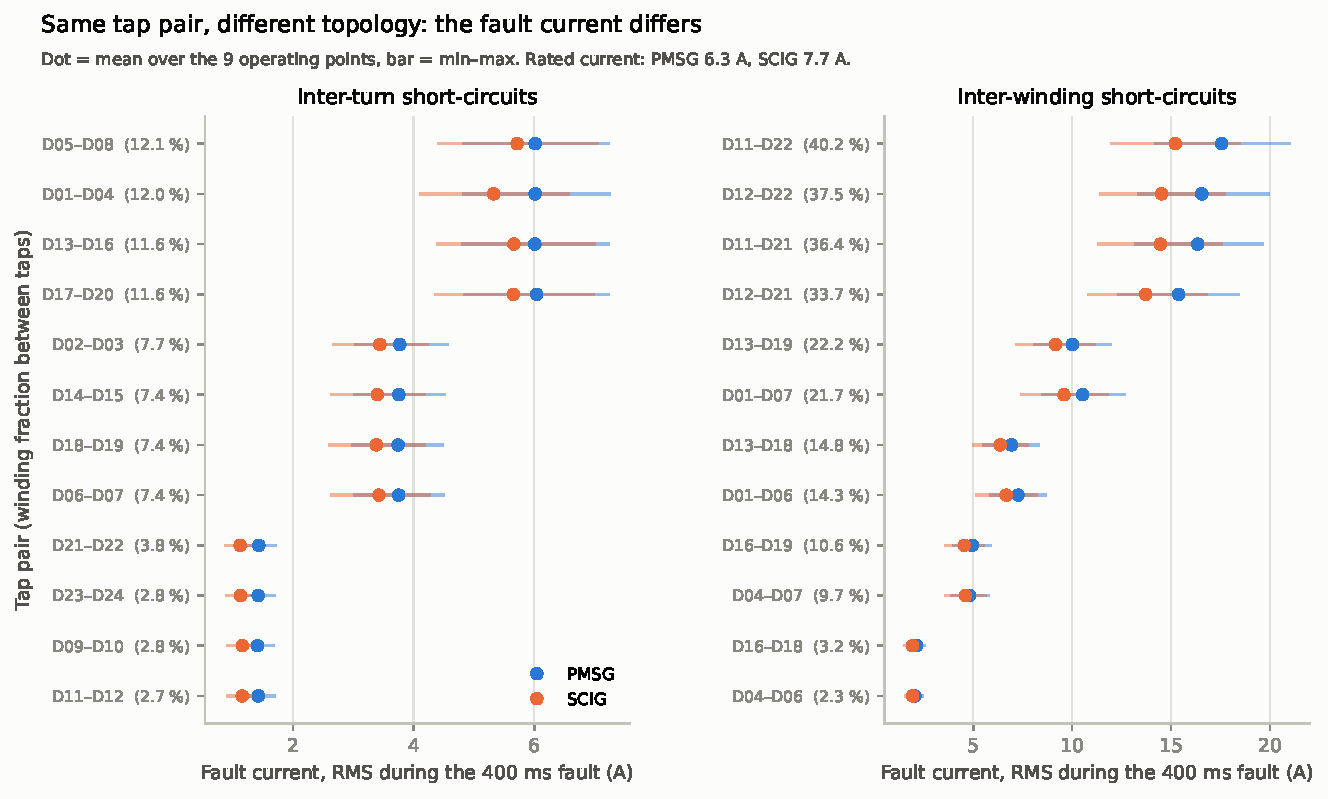
\includegraphics[width=\textwidth]{A_fault_current_by_case}
\caption{Fault current per tap pair, PMSG and SCIG: mean over the nine operating points (dot) and range (bar). Rated currents 6.3\,A (PMSG) and 7.7\,A (SCIG).}\label{fig:faultcurrent}
\end{figure}

\begin{figure}[t]
\centering
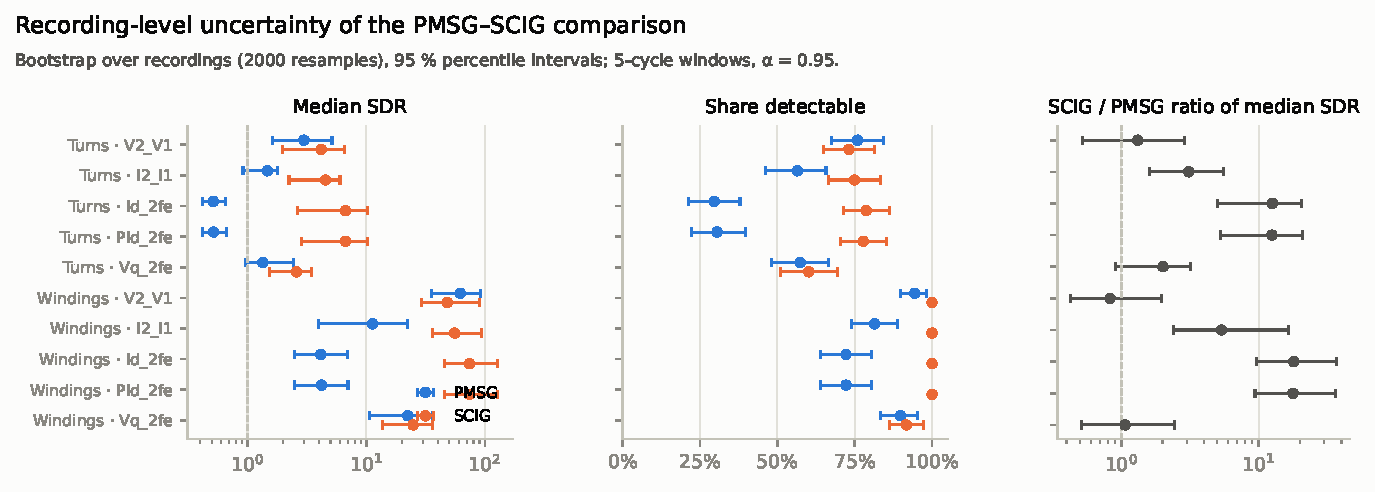
\includegraphics[width=\textwidth]{H_bootstrap}
\caption{Tap-pair-level uncertainty: bootstrap 95\,\% intervals of the median SDR, the detectable share and the SCIG/PMSG ratio of median SDR for five features and both fault classes (the same resampled tap pairs for both machines), five-cycle windows.}\label{fig:boot}
\end{figure}

\end{document}
